\documentclass[border=10pt]{standalone}
\usepackage{tikz}
\usetikzlibrary{positioning,quotes}
\begin{document}
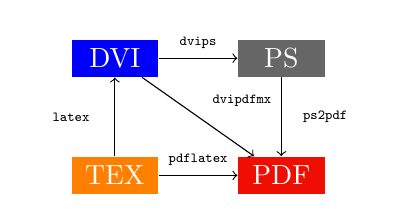
\begin{tikzpicture}[
    every node/.style = {text=white, minimum width = 1.1cm},
    every edge/.style = {draw,->},
    every edge quotes/.style = {auto, font=\tiny\ttfamily, text=black}]
  ]
  \node (tex) [fill=orange] {TEX};
  \node (pdf) [fill={rgb:red,244;green,15;blue,2},right = of tex] {PDF};
  \node (dvi) [fill=blue, above = of tex] {DVI};
  \node (ps)  [fill=black!60, above = of pdf] {PS};
  \draw (tex) edge["pdflatex"] (pdf);
  \draw (tex) edge["latex"]    (dvi);
  \draw (dvi) edge["dvips"]    (ps);
  \draw (dvi) edge["dvipdfmx"] (pdf);
  \draw (ps)  edge["ps2pdf"]   (pdf);
\end{tikzpicture}
\end{document}
